%! TEX root = ../../main.tex
\documentclass[../../main]{subfiles}

\begin{document}
\chapter{GPD赤道儀モータードライブ製作} % タイトル
\rightline{4年 森山 陽介} % 学年と名前(ハンドルネームでも可)
\section{概要}
電気通信大学天文部には実働する赤道儀が少ない。部で所有している赤道儀は9つあるが、実働しているのは屋上のNGT-18のホースシュー型赤道儀と、PENTAX 75SDHF望遠鏡に付属しているMS-3N赤道儀の2つだけである。
今回は、使える赤道儀を増やす試みの第1段階として、Vixen GPD赤道儀のモーターユニットをマイコンボードArduinoを使用して制御する手法および動作要件を検証した。
\section{背景}
\subsection{赤道儀とは}
\begin{wrapfigure}{r}[0pt]{.5\textwidth}
  \centering
  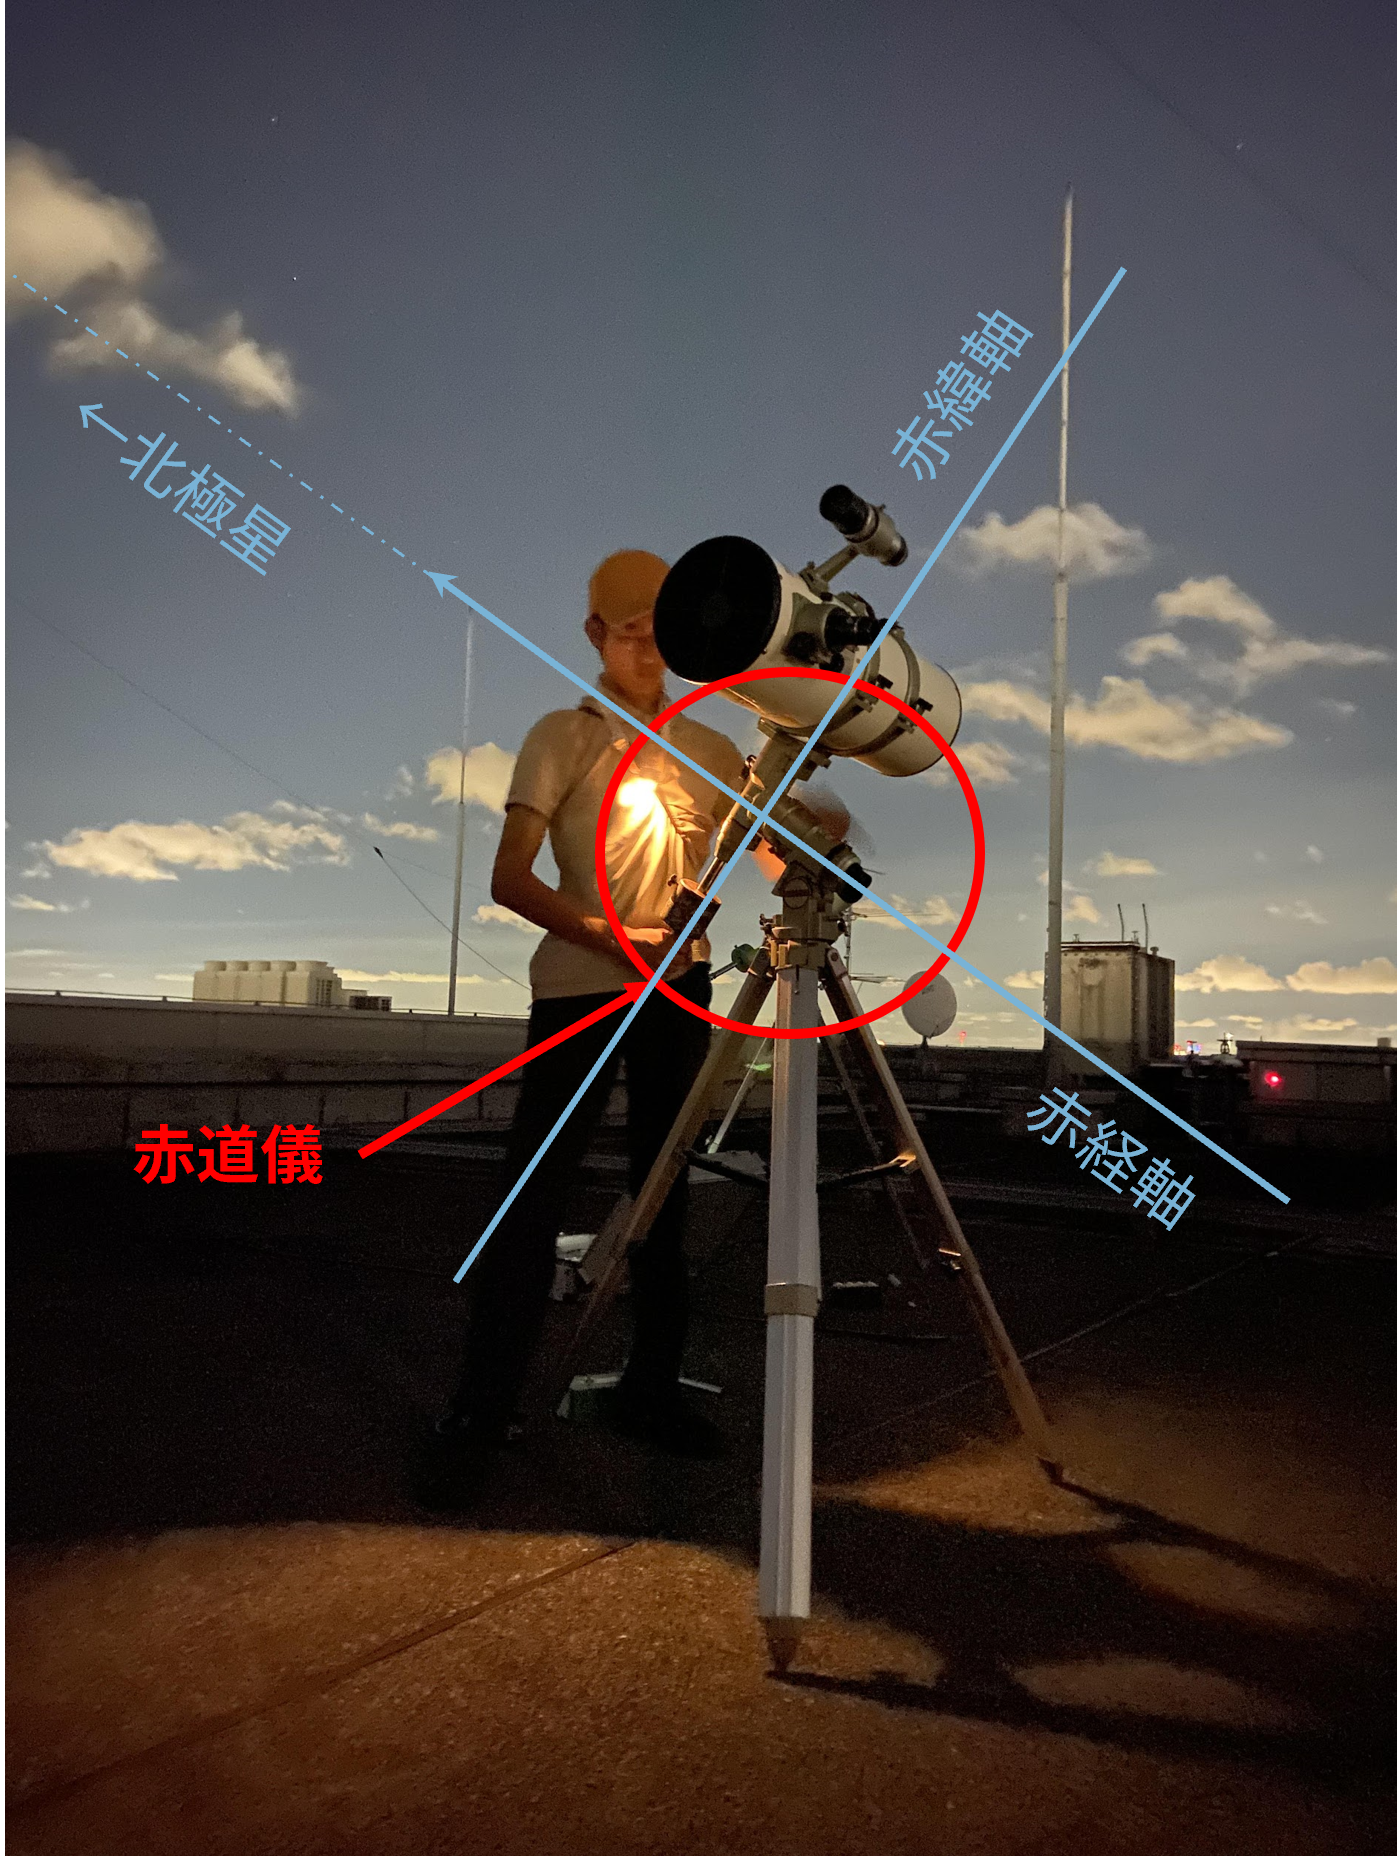
\includegraphics[width=.4\textwidth]{Equational_Mount.png}
  \caption{赤道儀}
  \label{fig:Equational_Mount}
\end{wrapfigure}
赤道儀とは、望遠鏡を載せる架台であり、天体を長焦点・長時間で観察や撮影をする際に必要となる。カメラと三脚を使ったことがある人であれば、三脚の雲台の1つと考えてもらえればよい。

赤道儀は赤経軸と赤緯軸の赤道座標系\footnote{天球座標系の1つ}に対応した赤経体と赤緯体の2つから構成されており、赤経体の中心軸を北極星付近にある天の北極(極軸)に合わせることで、地球の自転軸と平行になる。
太陽をはじめとする星や天体は、地球の自転によりこの天の北極(極軸)を中心として反時計回りに回転するように動いて見える。これを日周運動という。自転および日周運動は、1日に1回転することから、1時間に15$^\circ~(= 360^\circ \div 24)$のペースで回転している。
天体を追尾するためには、赤経体を1時間に15$^\circ$のペースで回転させ、日周運動と同調させる必要がある。
\begin{figure}
  \centering
  \includegraphics[width=.5\textwidth]{Move-Star.png}
  \caption{赤経体の回転の有り無しによる違い}
  \label{fig:Move-Star}
\end{figure}

この他に、赤経体を極軸に合わせるための水平方向と仰角方向への微動機構が備わっている。
\subsection{現代の赤道儀}
赤道儀の基本機能としては、赤経体の一軸を日周運動と同調させることで満足できる。現代においては、赤経体は専らステッピングモーターによって駆動されている。
更には、赤経体のみならず赤緯体もモーターに接続し、二軸をモーターで制御されているものが主流である。
これによりリモコンによる対恒星時数十倍速での粗動や数倍速での微動を行い、天体の導入や視野調整を可能にしている。
また最近では、PCなど天文データベースと接続することにより自動で天体を導入したり、ガイドカメラにより赤道儀の追尾エラー量をフィードバックするオートガイドなどの機能が一般的になりつつある。
\subsection{天文部所有の赤道儀}
電気通信大学天文部では、現在次の9つの赤道儀を保有している。
\begin{itemize}
  \item NGT-18ホースシュー型赤道儀
  \item PENTAX MS-3N赤道儀
  \item Vixen ATLUX赤道儀
  \item Vixen GPD赤道儀(エンコーダー付)
  \item Vixen GPD赤道儀(ノーマル)
  \item タカハシ システム90赤道儀
  \item タカハシ EM-100赤道儀
  \item 五藤光学 マークX赤経体(2台)
\end{itemize}
このうち、実働しているのはNGT-18ホースシュー型赤道儀とPENTAX MS-3N赤道儀の2つであり、NGT-18は屋上備付けの大型反射望遠鏡であるため、合宿・遠征へ持ち出しが可能な赤道儀はMS-3N赤道儀のみとなる。
このMS-3N赤道儀は、小型であるため搭載可能重量が小さく、実質付属のPENTAX 75SDHF望遠鏡専用品となっているのが現状である。

天文部所有の各種望遠鏡を搭載し、天体観測および撮影をするためには、これら2つ以外の赤道儀を使用する必要があるが、モーターの欠損や歯車の脱落、制御装置の紛失などにより、稼働できる状態にない。
幸いにも、大枠部分の機構および強度には問題が見られないため、駆動装置の取り付けと制御が行えれば、使用可能であると見込まれている。
\section{今回の対象となる赤道儀}
\begin{wrapfigure}{r}[5pt]{.3\textwidth}
  \centering
  \includegraphics[width=.3\textwidth]{GPD.jpg}
  \caption{GPD赤道儀}
  \label{fig:GPD}
\end{wrapfigure}
今回の検証に用いるのは、Vixen GPD赤道儀になる。この赤道儀はモーターユニットMT-1と、モーター接続と手動ハンドルの接続を切り替えられる「粗動クラッチ」が残っている。
そのため、動作検証の第一歩に用いるのに最適であると考えた。

GPD赤道儀の駆動制御に当たっては汎用マイコンボードArduinoを用いて行う。
\subsection{モーターの仕様}
Arduinoを接続し、制御するに当たっては、モーターの駆動原理を理解する必要がある。MT-1モーターユニットを分解し、中身のステッピングモーターと配線を確認したところ、ステッピングモーターは日本パルスモーター製の「PF42-48I3」、配線は6本あり「黒・橙・赤・赤・黃・茶」であった。
\begin{figure}
  \centering
  \begin{minipage}{0.4\columnwidth}
    \centering
    \includegraphics[width=\columnwidth]{motor.jpg}
    \caption{ステッピングモーター}
    \label{fig:motor}
  \end{minipage}
  \begin{minipage}{0.4\columnwidth}
    \centering
    \includegraphics[width=\columnwidth]{pin.png}
    \caption{配線の様子}
    \label{fig:pin}
  \end{minipage}
\end{figure}
ステッピングモーターの概要を調べたところ以下のような仕様(\figref{PF42})・動作原理(\figref{detail})であることがわかった。
\begin{figure}[H]
  \centering
  \includegraphics[width=.8\textwidth]{PF42.png}
  \caption{型番から読める仕様}
  \label{fig:PF42}
\end{figure}
\begin{figure}
  \centering
  \includegraphics[width=.8\textwidth]{detail.png}
  \caption{動作原理}
  \label{fig:detail}
\end{figure}
ステッピングモーターは、モーターの軸に交互に配置されたN極とS極が、四方に囲まれたコイルが電磁石としてN極とS極を交互に入れ替えることで、回転を行う。今回のモーターでは、「黒・茶・橙・黃」のケーブルにかかる電圧のON/OFFを\figref{detail}のシーケンスに沿って制御することで、
1シーケンスごとに7.5$^\circ$ずつ回転する。赤道儀では、超低速で高トルクを得るために減速ギアが取り付けられており、出力される回転量は1/120となる。
\subsection{回路の構成}
シーケンスの制御には、NPNトランジスタを用いたスイッチング回路(\figref{circuit})を4つ作成し、それぞれモーターの「黒・茶・橙・黃」の線とArduinoのGPIO端子「10・11・12・13」に接続した。
\begin{figure}[H]
  \centering
  \begin{minipage}{0.4\columnwidth}
    \centering
    \includegraphics[width=\columnwidth]{circuit.png}
    \caption{スイッチング回路}
    \label{fig:circuit}
  \end{minipage}
  \begin{minipage}{0.4\columnwidth}
  \centering
    \includegraphics[width=\columnwidth]{bread-board.png}
    \caption{ブレッドボードに回路を組んだ様子}
    \label{fig:bread-board}
  \end{minipage}
\end{figure}
\subsection{回転速度の導出および制御}
\begin{wrapfigure}{r}[0pt]{.4\textwidth}
  \centering
  \includegraphics[width=.3\textwidth]{gear.png}
  \caption{ウォームホイールとモーターの関係}
\end{wrapfigure}
ステッピングモーターのシーケンス表を基にArduinoに組み込んだプログラムはListing\ref{code1}のようになる。

switch文とfor文により各シーケンスが順番に実行されている。ここで、48行目のdelay値がモーターの回転速度に直結する値になり、日周運動と同期する15$^\circ$/hの回転速度となるように設定をしなくてはならない。
赤経体に取り付けられているウォームホイールと呼ばれる大きな歯車の歯の数は144個$^{\cite{DIY}}$であり、ウォームギアが1回転することで、$\theta = 2.5^\circ (= 360^\circ \div 144)$回転することになる。
つまり、日周運動と同期するためにはウォームギアおよびモーターは1時間に6回転、すなわち1回転に10分(600秒)となる必要がある。

モーターのステップ角が7.5$^\circ$、ギア比が1/120であることから
\[ \frac{600 \times 10^3 \si{[ms]}}{120 \times (360^\circ / 7.5^\circ) \text{[回転]}} = 104.6 \si{ms} \]

\begin{tcolorbox}[title=, breakable]
\lstinputlisting[caption=作成したプログラム, label=code1]{sketch_aug27a.ino}
\end{tcolorbox}
\section{プロトタイプ試験}
\subsection{試験概要}
ユニバーサル基板に回路を実装し、8ピンDIN端子と6軸ケーブルを取り付け、プロトタイプとして、赤道儀に取り付けできる形にした。
\begin{figure}[H]
  \centering
  \begin{minipage}{0.4\columnwidth}
    \centering
    \includegraphics[width=\columnwidth]{prototype1.jpg}
    \caption{ユニバーサル基板への実装}
    \label{fig:prototype1}
  \end{minipage}
  \begin{minipage}{0.4\columnwidth}
    \centering
    \includegraphics[width=\columnwidth]{prototype2.jpg}
    \caption{プロトタイプの外観}
    \label{fig:prototype2}
  \end{minipage}
\end{figure}
このプロトタイプ機を用いてGPD赤道儀にて動作試験を行った。
方法としては、R200SS反射望遠鏡とFC-76屈折望遠鏡を取り付け、カメラで30秒露光したときの星像の流れ具合を確認する。本来ならばきちんとした極軸合わせのもと行うべきだが、{\bfseries 諸般の都合により}、今回は大雑把な極軸合わせの条件下となる。
\begin{figure}
  \centering
  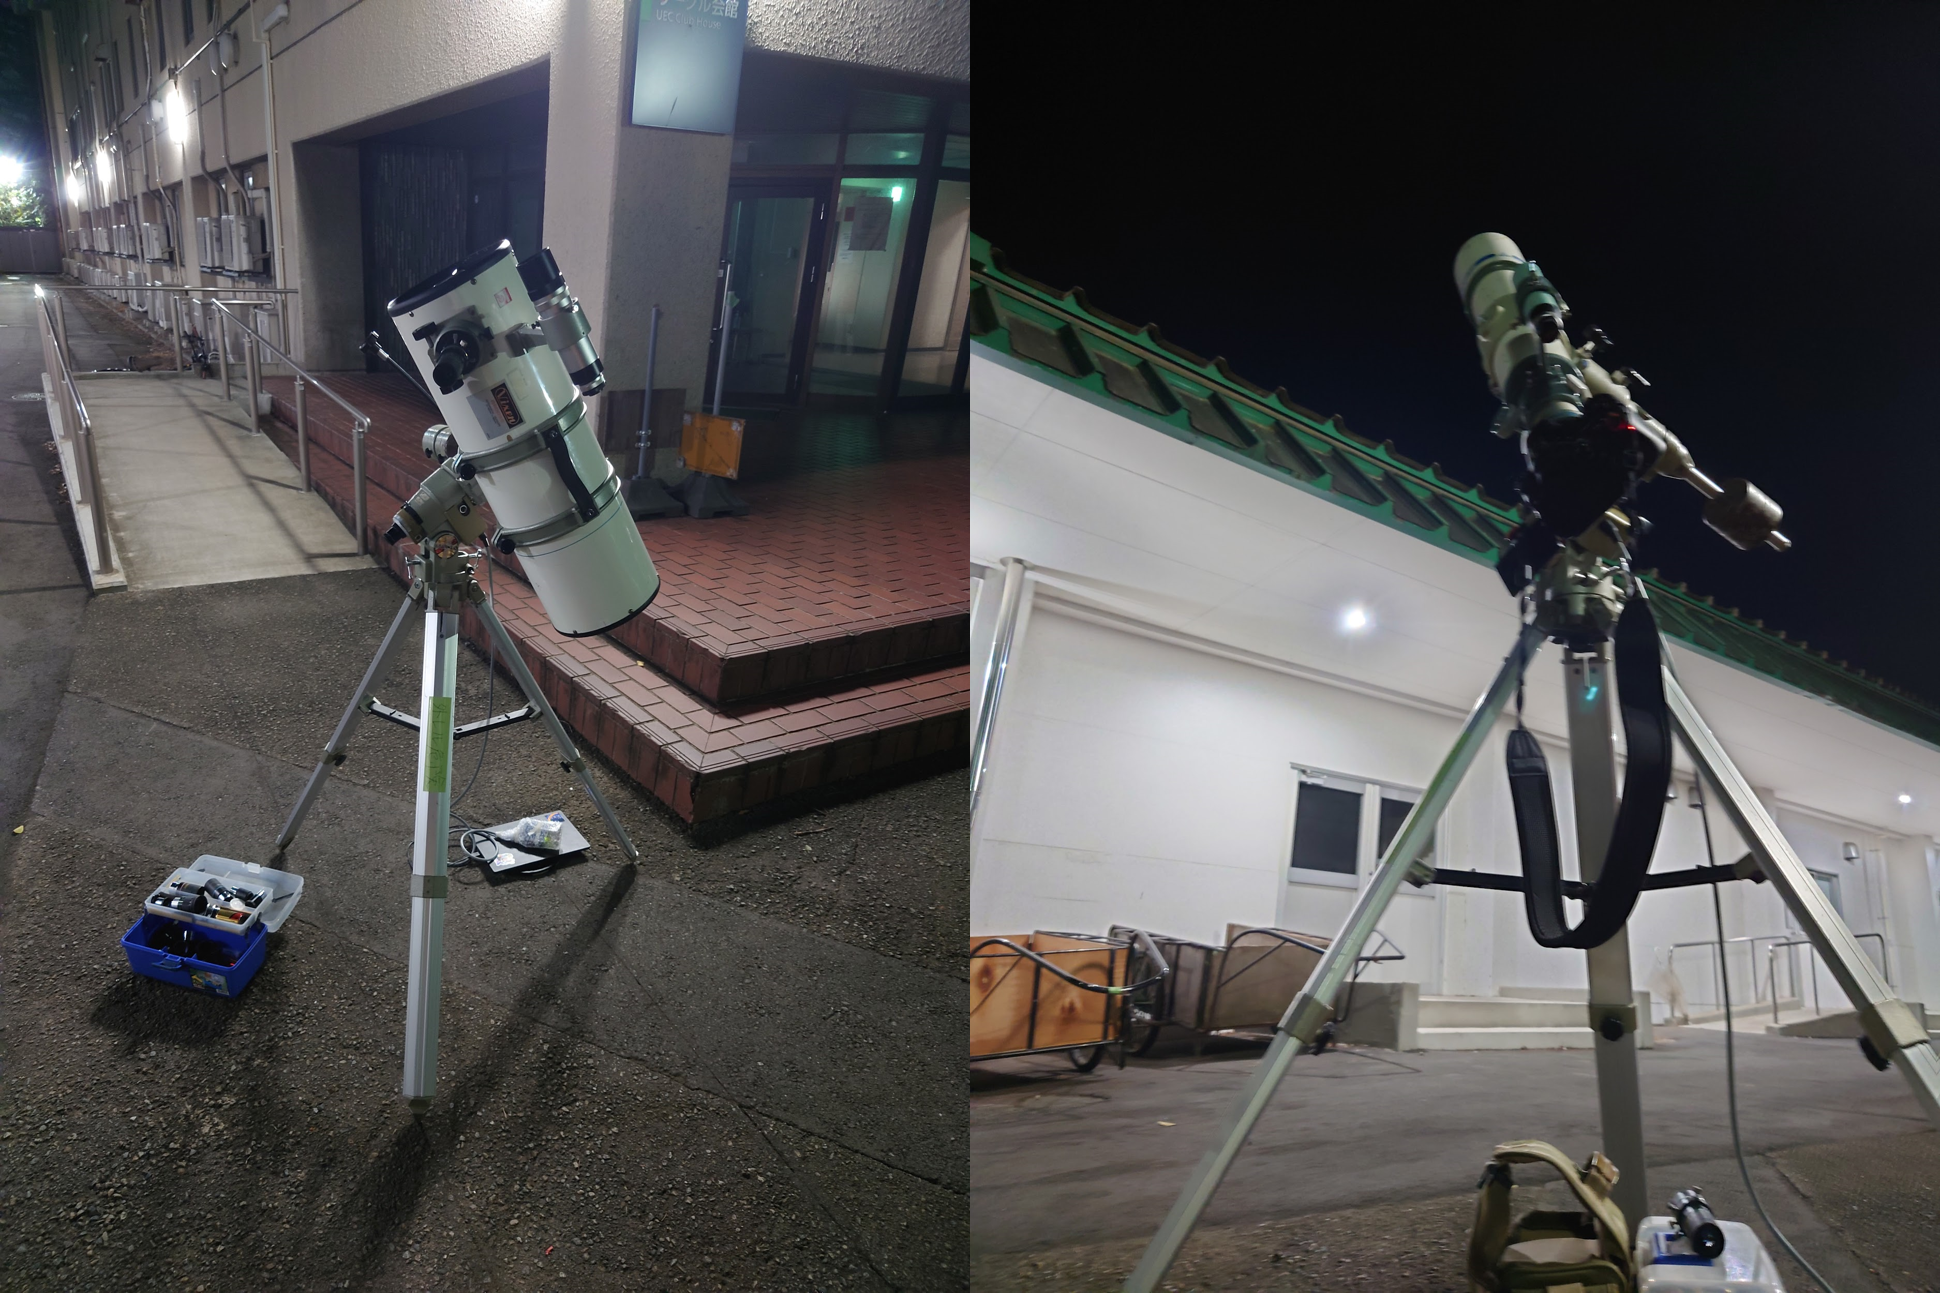
\includegraphics[width=.5\textwidth]{experiment.png}
  \caption{試験の様子}
  \label{fig:experiment}
\end{figure}
\subsection{試験結果}
結果は次の様になる。
\begin{figure}[H]
  \centering
  \begin{minipage}{0.4\columnwidth}
    \centering
    \includegraphics[width=\columnwidth]{R200SS.png}
    \caption{R200SSでの星像}
    \label{fig:R200SS}
  \end{minipage}
  \begin{minipage}{0.4\columnwidth}
    \centering
    \includegraphics[width=\columnwidth]{FC-76.png}
    \caption{FC-76.png}
    \label{fig:FC-76}
  \end{minipage}
\end{figure}
R200SSでは大きく星が流れているのにたいして、FC-76ではそこまで大きく流れていない。また、流れている方向に関しては、赤経体を回転させたときの方向とは異なっていることがわかっている。
これらを踏まえると、FC-76といった軽量な鏡筒の場合はある程度日周運動と同期しているように見えるが、R200SSといった重量のある場合には脱調などパワー不足が原因で日周運動と同期できていないと考えられる。
\section{今後について}
今回の結果から見えたパワー不足の原因としては、電源電圧がArduinoからの5Vのみであることが大きいと考えられる。本来の赤道儀は12Vで稼働することが一般的であるため、モーターへの電源として別途12Vの電源を用いる必要がある。
電源の候補としては、PD対応モバイルバッテリーから12Vトリガーケーブルを利用するのが妥当だろう。また、12Vを入れるに当たって、もう一度回路の抵抗値などを見直す必要もありそうだ。

また、調べを進めていくうちに最近での同様の試みがネット上に見られている。これらの内容をよく見て改良を加えていきたい。

\vspace{2\zw}
\begin{figure}
  \centering
  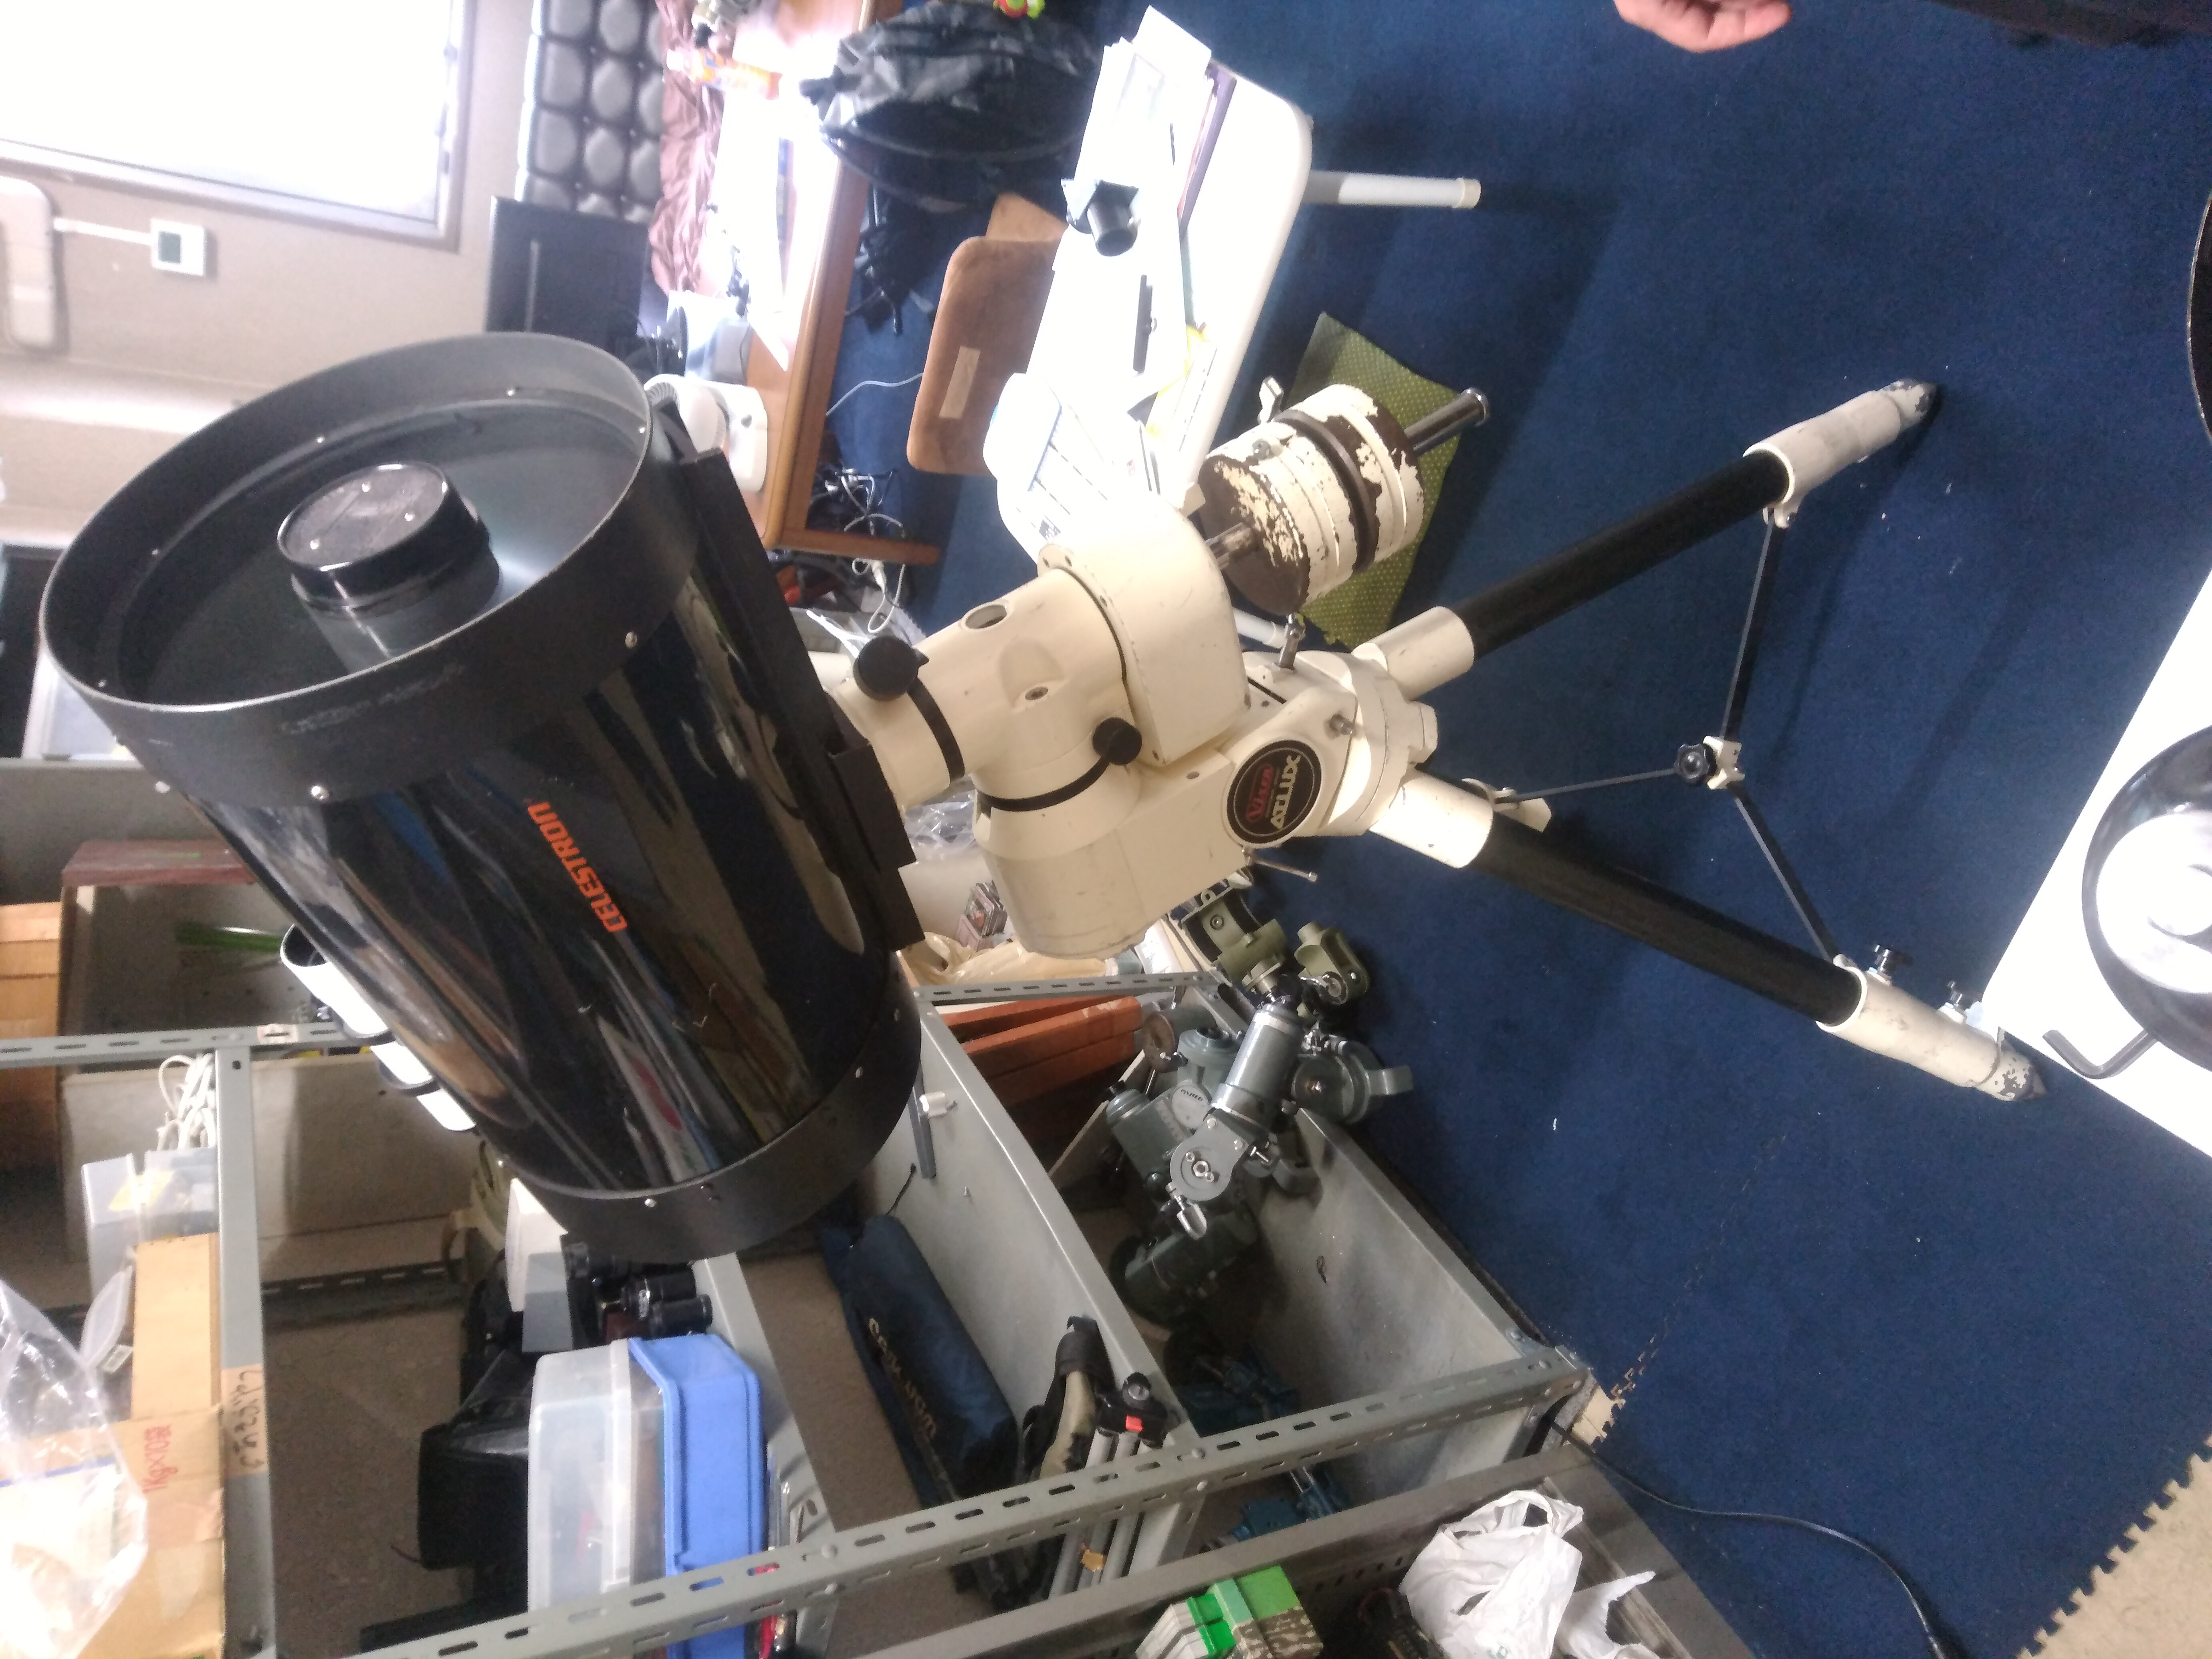
\includegraphics[width=.8\textwidth, angle=-90]{DSC_1020.jpg}
  \caption{\Large いつかはATLUX赤道儀を動かすぞ!!}
  \label{fig:ATLUX}
\end{figure}

\begin{thebibliography}{9}
  \bibitem{NPN} 
  トランジスタのスイッチング回路, 始める電子回路, \url{https://startelc.com/elc/elc_3_7Tr2sw.html}
  \bibitem{DIY} 
  DIY controller for Nippon PF42-48 motor specs wanted, STARGAZERS LOUNGE, \url{https://stargazerslounge.com/topic/367892-diy-controller-for-nippon-pf42-48-motor-specs-wanted/}
  \bibitem{MT-1}
  MT-1モーターをUSB-IOで動かす, 天文我楽苦多工房, \url{http://garakutakohbo.web.fc2.com/labo/mt-1/mt1.htm}
  \bibitem{GPD}
  GPD赤道儀基礎知識まとめ, pirosap.tech, \url{https://astronomy.pirosap.tech/ja/gpd/gpd-basics}
\end{thebibliography}
\end{document}
